\documentclass[10pt,a4paper]{article}
\usepackage[utf8]{inputenc}
\usepackage{amsmath}
\usepackage[margin=1.25in]{geometry}
\usepackage[pdftex]{graphicx}
\usepackage{amsfonts}
\usepackage{amssymb}
\usepackage{hyperref}
\hypersetup{
    colorlinks=true,
    citecolor=black,      
    urlcolor=cyan,
}
\usepackage[T1]{fontenc}
\usepackage{listings}
\renewcommand*{\figurename}{Rys.} 
\renewcommand*{\tablename}{Tab.} 
\author{Rafał Kornel}
\title{\textbf{Symulacje dynamiki molekularnej - ruchy planet.}}
\date{}
\begin{document}
\maketitle




\section*{Wstęp}
	Problem - rozwiązać numerycznie problem dwóch ciał.
	\begin{equation} \textbf{F}_{j} = m_{j} \frac{d^{2}\textbf{r}_{j}}{dt^2} = \sum_{i = 1, i \neq j}^{N} \textbf{F}_{ij} \end{equation}
	
	Do rozwiązania problemu zostały użyte trzy metody numeryczne:
	
\subsection*{Algorytm Eulera}
	Wynika z rozwinięcia w szereg Taylora:
	\begin{equation} \textbf{r}(t+\delta t) \approx \textbf{r}(t) + \dot{\textbf{r}}(t) \delta t +\frac{1}{2!} \ddot{\textbf{r}}(t) \delta t^2	\end{equation}
	
	Stąd wynikają wzory na położenie oraz pęd:
	$$ r(t + \delta t) = r(t) + p(t) \delta t + \frac{1}{2} F(t) \delta t^2 $$
	$$ p(t + \delta t) = p(t) + F(t) \delta t $$
	
	Kod poniżej przedstawia klasę, która została użyta do przechowywania danych.	
	
\lstset{language=Python}
\lstset{label={lst:code_direct}}
\lstset{basicstyle=\footnotesize}
\lstset{keywordstyle=\color{blue}}
\lstset{commentstyle=\color{green}}
\lstset{stringstyle=\color{red}}

\begin{lstlisting}
class Planet:
    def __init__(self, pos, mom, m, static = False):
        self.pos = pos			# position
        self.mom = mom			# momentum
        self.m = m			# mass
        self.pos_history = []
        self.vel_history = []
        self.pot = []			# potential energy
        self.kin = []			# kinetic energy
        
        self.is_static = static
        self.r = 0.3 if static else 0.2
        self.fig = pl.Circle( self.pos, self.r, color=pl.cm.summer(self.m))
   
\end{lstlisting}


	Kod poniżej przedstawia implementacje algorytmu Euler'a.

\begin{lstlisting}
def evolve_euler(self):
        for p in self.planets:
            f = self.calculate_force(p)

            p.pos_history.append(p.pos)
            
            kin, pot = self.calculate_energy(p)
            p.kin.append(kin)
            p.pot.append(pot)
            
            p.pos = p.pos + p.mom * self.dt/p.m + 1/(2*p.m) * f * (self.dt**2)
            p.mom = p.mom + f * self.dt
\end{lstlisting}

	Dla $N = 100000$ iteracji, orbita planety o warunkach początkowych
	$$ \textbf{r} = (2, 0) $$
	$$ \textbf{p} = (0, 0.1) $$
	wygląda następująco:

	\begin{figure}[htp!!!!!!]	
		\begin{center}
			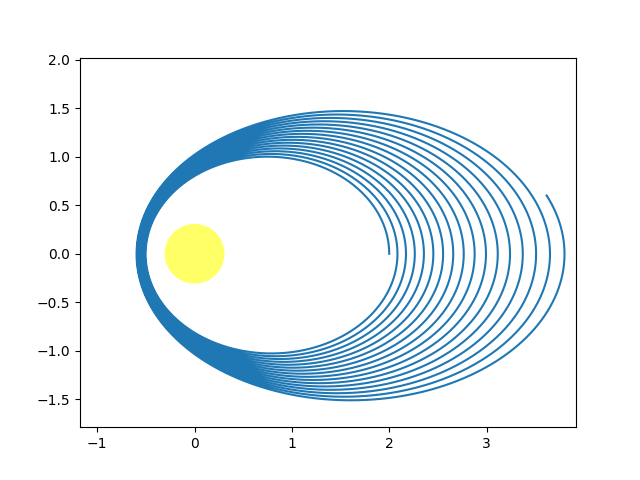
\includegraphics[width = 0.9\textwidth]{euler_orbit.png}
			\caption{Orbita planety w metodzie Eulera.}
			\label{schemat}
		\end{center}
	\end{figure} 

	A tak wygląda wykres energii:

	\begin{figure}[htp!!!!!!]	
		\begin{center}
			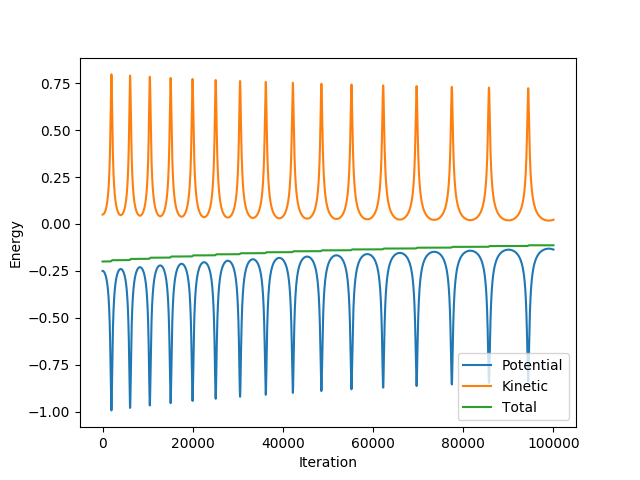
\includegraphics[width = 0.9\textwidth]{euler_energy.png}
			\caption{Bilans energii w symulacji metoda Eulera.}
			\label{schemat}
		\end{center}
	\end{figure} 
	
	Energia całkowita w tej metodzie nie jest zachowana, co widać na przybliżeniu:
	\begin{figure}[htp!!!!!!!!]	
		\begin{center}
			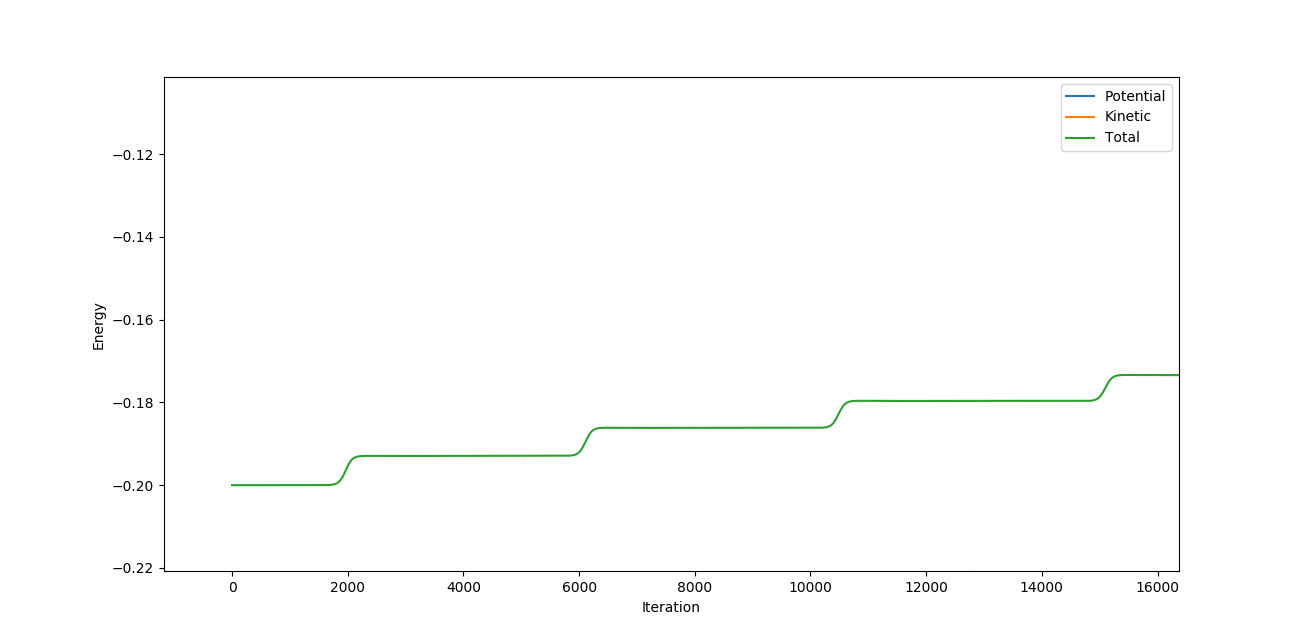
\includegraphics[width = 0.9\textwidth]{euler_energy_closeup.png}
			\caption{Przybliżenie wykresu energii - widać wzrosty energii całkowitej.}
			\label{schemat}
		\end{center}
	\end{figure} 
	
\subsection*{Algorytm Verleta}
	Wzór na położenie w n-tym kroku ma następującą postać:
	$$ r_{n+1} = 2r_{n} - r_{n-1} + ( \frac{F_{n}}{m}) \delta t^2 $$
	Jak widać, do wyznaczenia n+1-ego kroku potrzebujemy tylko n-tego i n-1-ego położenia.
	Prędkość nie jest potrzebna do algorytmu Verleta, lecz gdybyśmy chcieli ją policzyć, 
	to wyraża się wzorem:
	$$ v_{n} = \frac{r_{n+1} - r_{n-1}}{2 \delta t} $$
	
	Tak wygląda implementacja algorytmu Verleta:
	
	\begin{figure} [htp!]
	\begin{lstlisting}
def evolve_verlet(self):
        for p in self.planets:
            f = self.calculate_force(p)

            if len(p.pos_history) == 0:
                pos_prev = p.pos - p.mom * self.dt/p.m
                p.pos_history.append(pos_prev)

            p.pos_history.append(p.pos)

            kin, pot = self.calculate_energy(p)
            p.kin.append(kin)
            p.pot.append(pot)

            p.pos = 2*p.pos_history[-1] - p.pos_history[-2] + f*(self.dt)**2/p.m
            p.mom = p.m/(2*self.dt) * (p.pos - p.pos_history[-2])
\end{lstlisting}
	\end{figure}
		
	
	Dla takich samych jak wyżej warunków początkowych orbita przy algorytmie Verleta 
	wygląda tak:
	
	\begin{figure}[htp!!!!!!!]	
		\begin{center}
			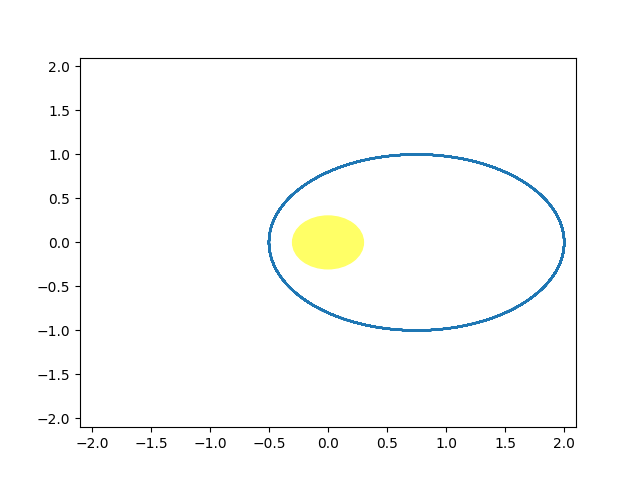
\includegraphics[width = 0.9\textwidth]{verlet_orbit.png}
			\caption{Orbita planety używajac algorytmu Verleta.}
			\label{schemat}
		\end{center}
	\end{figure} 

	Tak prezentuje się wykres energii w tymże algorytmie:
	
	\begin{figure}[htp!!!!!!!]	
		\begin{center}
			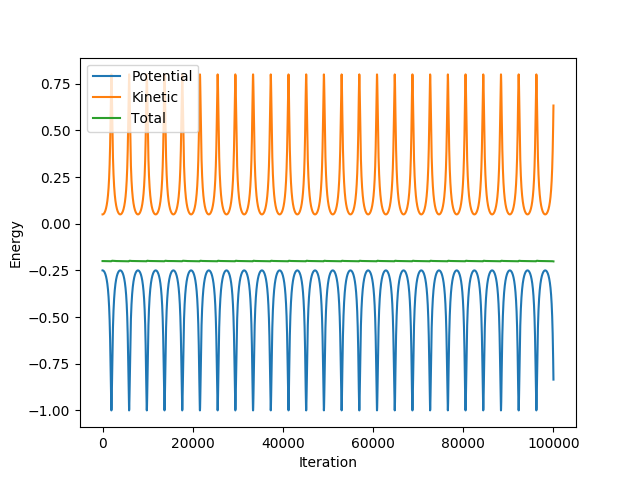
\includegraphics[width = 0.9\textwidth]{verlet_energy.png}
			\caption{Bilans energii w symulacji wykorzystując algorytm Verleta.}
			\label{schemat}
		\end{center}
	\end{figure} 

	Przybliżając wykres energii możemy zauważyć, że energia całkowita , mimo że nie jest 
	stała, to nie rośnie wraz z postępem symulacji. 
	
	\begin{figure}[htp!!!!!!!]	
		\begin{center}
			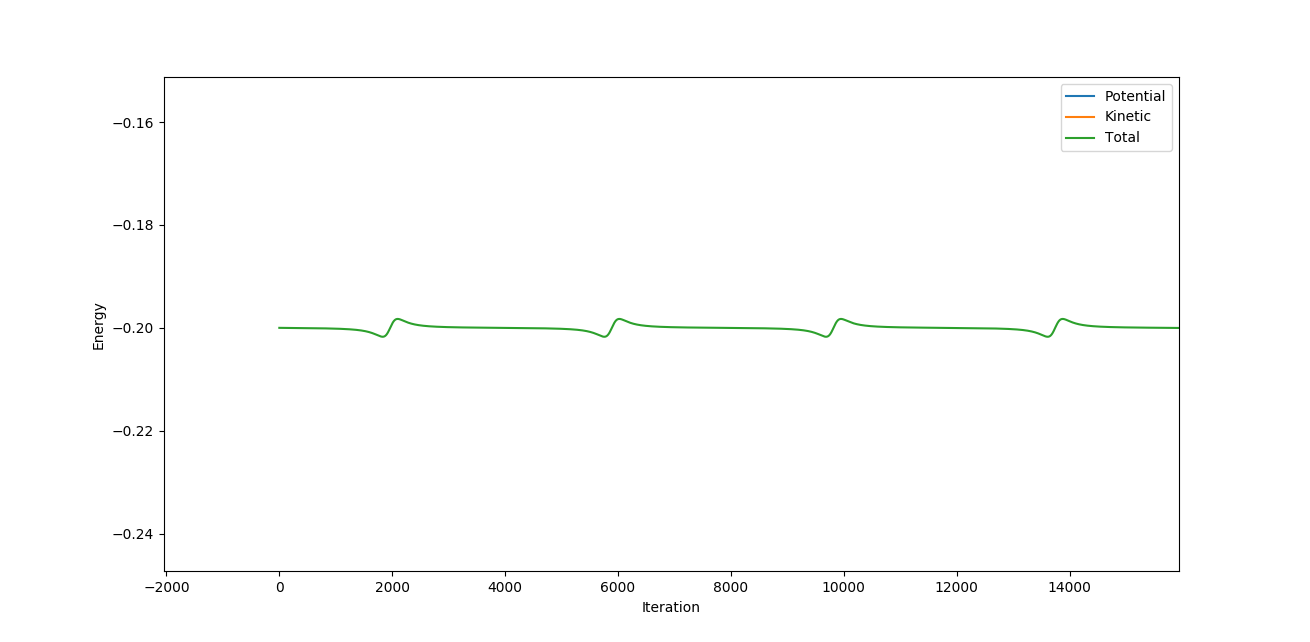
\includegraphics[width = 0.9\textwidth]{verlet_energy_closeup.png}
			\caption{Przybliżenie wykresu energii w metodzie wykorzystującej 
					 algorytm Verleta}
			\label{schemat}
		\end{center}
	\end{figure} 
	
\subsection*{Algorytm skokowy (leapfrog)}
	W algorytmie skokowym liczymy prędkość w kroku $n + 1/2$, aby uzyskać
	położenie. Wzory potrzebne do przeprowadzenia symulacji:
	$$ v_{n + 1/2} = v_{n - 1/2} + (\frac{F}{m})\delta t $$
	$$ r_{n + 1} = r_{n} + v_{n + 1/2} \delta t $$
	Kod przedstawiający implementacje algorytmu skokowego:
	
	\begin{lstlisting}
def evolve_leapfrog(self):
        for p in self.planets:
            f = self.calculate_force(p)

            if len(p.vel_history) == 0:
                p.vel_history.append(p.mom/p.m - f*self.dt/(2*p.m))

            p.pos_history.append(p.pos)
            p.vel_history.append(p.vel_history[-1] + f*self.dt/p.m)

            kin, pot = self.calculate_energy(p)
            p.kin.append(kin)
            p.pot.append(pot)
            
            p.mom = p.m*(p.vel_history[-1] + p.vel_history[-2])/2
            p.pos = p.pos + p.vel_history[-1]*self.dt
	\end{lstlisting}	
	
	Tak prezentuje się orbita planety w symulacji wykorzystującej algorytm skokowy:
	
	\begin{figure}[htp!!!!!!!]	
		\begin{center}
			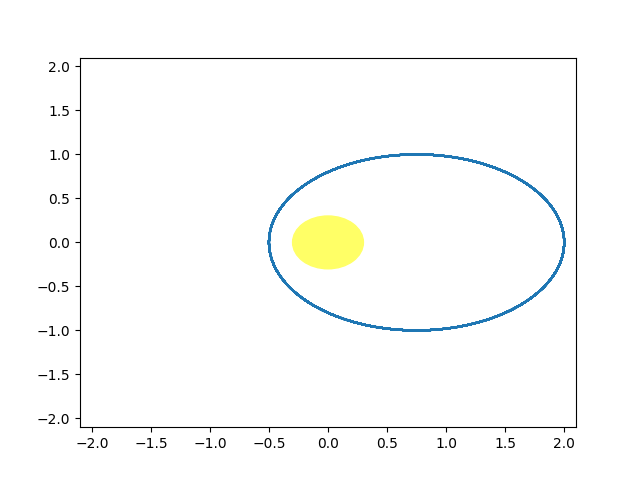
\includegraphics[width = 0.9\textwidth]{leapfrog_orbit.png}
			\caption{Orbita planety używajac algorytmu leapfrog.}
			\label{schemat}
		\end{center}
	\end{figure} 	
	
	Wykres energii w algorytmie leapfrog:
	
	\begin{figure}[htp!!!!!!!]	
		\begin{center}
			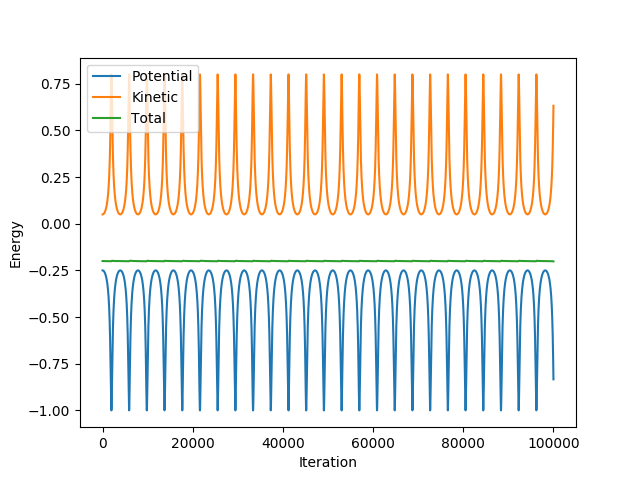
\includegraphics[width = 0.9\textwidth]{leapfrog_energy.png}
			\caption{Bilans energii w symulacji wykorzystując algorytm leapfrog.}
			\label{schemat}
		\end{center}
	\end{figure} 
	
	Przybliżając wykres energii możemy zauważyć, że tutaj, podobnie jak w przypadku
	algorytmu Verleta, energia nie jest zachowana, lecz nie rośnie nieograniczenie.
	
	\begin{figure}[htp!!!!!!!]	
		\begin{center}
			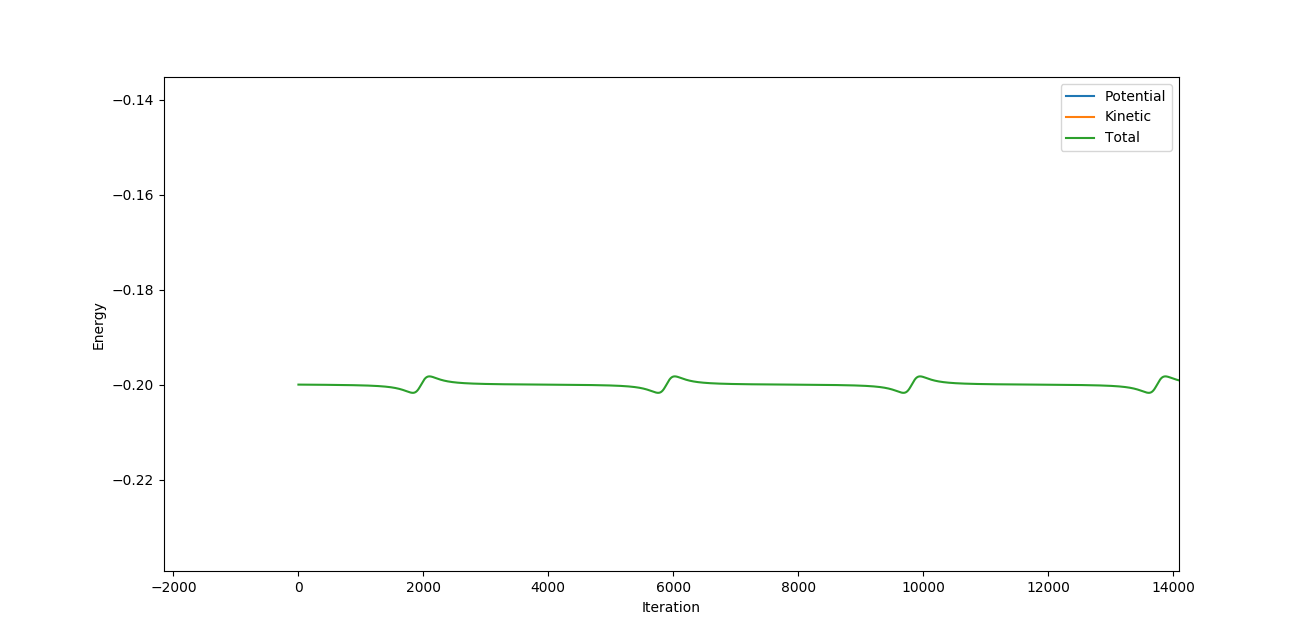
\includegraphics[width = 0.9\textwidth]{leapfrog_energy_closeup.png}
			\caption{Przybliżenie wykresu energii w metodzie wykorzystującej 
					 algorytm leapfrog}
			\label{schemat}
		\end{center}
	\end{figure} 
	
	
\subsection*{Próby uzyskania lemniskaty Chencinera}
Niestety, nie udało się uzyskać orbity w kształcie lemniskaty, mimo zastosowania
podanych w pracy \cite{zrodlo1} warunków początkowych. Poniżej zostały przedstawione 
otrzymane rezultaty:

\begin{figure}[htp!!!!!!!]	
		\begin{center}
			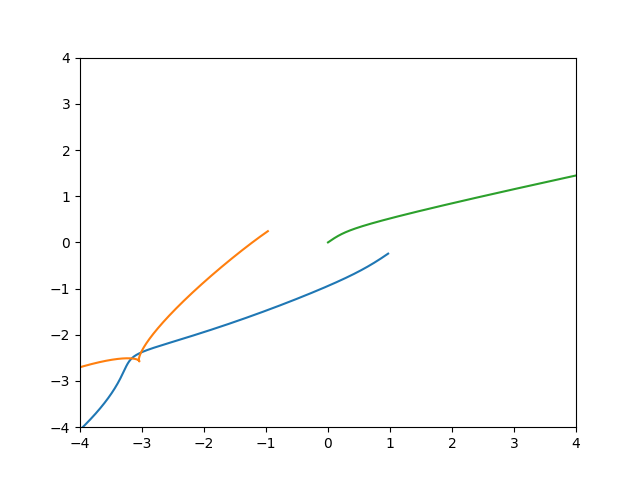
\includegraphics[width = 0.9\textwidth]{osemka_chencinera.png}
			\caption{Symulacja przeprowadzona dla warunków początkowych przedstawionych
					w pracy Chencinera.}
			\label{schemat}
		\end{center}
	\end{figure} 
		
	
\subsection*{Inne metody / fragmenty kodu użyte w symulacji}
Klasa World - piaskownica symulacji:
\begin{lstlisting}
class World:
	def __init__(self, G, planets, static_objects, dt):
		self.G = G
		self.planets = planets
		self.statics = static_objects
		self.dt = dt
		self.size = 2.1
\end{lstlisting}	
	
Metoda licząca siłę, działającą na cząstkę:	
	
\begin{lstlisting}
def calculate_force(self, planet):
        f = np.array([0., 0.])

        for other in self.planets + self.statics:
            if planet is not other:
                d = World.d(other.pos, planet.pos)
                f +=  ( self.G * planet.m * other.m / d**3 )\
                     * (other.pos - planet.pos)

        return f
\end{lstlisting}	
	
Metoda licząca energię kinetyczną i potencjalną cząstki:
\begin{lstlisting}
def calculate_energy(self, p):
        pot = 0
        for o in self.planets + self.statics:
            if p is not o:
                pot += (-1) * self.G * o.m * p.m / World.d(o.pos, p.pos)
        kin = 0.5 * np.linalg.norm(p.mom) ** 2 / p.m
        return (kin, pot)
\end{lstlisting}	

Metoda licząca odległość między dwiema cząsteczkami:
\begin{lstlisting}
@staticmethod
def d(r1, r2):
        dist = ( (r1[0] - r2[0])**2 + (r1[1] - r2[1])**2  )**0.5
        return dist
\end{lstlisting}	
	
	
\begin{thebibliography}{}
	\bibitem{zrodlo1} Oryginalna praca Chencinera 
	http://emis.matem.unam.mx/journals/Annals/152{\_}3/chencine.pdf 
\end{thebibliography}
	
\end{document}